\documentclass[10pt,letterpaper]{article}
\usepackage[english]{babel}
\usepackage[utf8]{inputenc}
\usepackage[T1]{fontenc}
\usepackage{geometry}
\usepackage{amsmath,amssymb,hyperref,xcolor,booktabs,array}
\usepackage{caption}
\usepackage{float}
\usepackage{pgfplots}
\pgfplotsset{compat=1.17}
\geometry{top=1in,bottom=1in,left=1in,right=1in}

\title{\textbf{Report}\\[0.2cm]
\large Caption-Quality and Shot-Boundary Evaluation of a Video-Curation Pipeline}
\author{}
\date{2026-06-26}

\begin{document}

\maketitle

\section{Background and contributions}

\textbf{Caption-quality evaluation.} The primary contribution is a caption-evaluation harness,
built over the preceding week and run end-to-end on the full 2{,}587-video AgiBot set, that scores
semantic grounding, judge reliability, adjacent-window consistency, and a single composite quality
score across every video split. It corrects three flaws in the prior evaluation. Temporal
grounding was unsound: each $\sim$8.5\,s window was assigned a \emph{single} majority-overlap
ground-truth action, so in multi-action windows (a pick followed by a place) the minority action
was discarded, penalising transition-aware captions while letting incomplete captions pass; the
ground-truth source now returns \emph{all} overlapping actions with per-window coverage and a
transition flag, and multi-label precision, recall, and F1 weight each action equally. The judges
were either weak (a text-only Gemma4 variant) or niche (a LoRA fine-tune of Qwen2.5-VL) and
reported only a single 1--5 score; a Qwen3-VL-30B-A3B mixture-of-experts judge was added with
structured outputs that assess object- and action-correctness separately, behind a
configuration-driven loader. Grounding also relied purely on lexical (bag-of-words) overlap, which
missed paraphrases and rewarded verbosity; clause-level semantic grounding with a sentence-embedding
model now matches each ground-truth action to its best clause, a precision term penalises
unsupported content, and a length-robustness diagnostic confirms scores cannot be inflated by
writing more.

Beyond these fixes, the harness reports cross-judge agreement (Cohen's $\kappa$), sub-action
completeness, caption uniqueness (folded into the composite score to discourage repetition), and
compute efficiency, producing a per-model ranking. The aim is a fair, comprehensive comparison of
captioning models and judges --- especially on multi-action and transition-heavy windows where
minority actions are no longer ignored --- that rewards captions which are both grounded and concise
while exposing models that lean on verbosity or repetition. The remaining steps are to run the
harness over additional model outputs and, where needed, re-caption and re-judge so that the
lexical-versus-semantic and single-label-versus-multi-label differences can be quantified directly.

\textbf{Shot-boundary segmentation (parallel component).} The segmentation side of the pipeline was
implemented as three classes of detector. Class~A is traditional shot-boundary detection used as a
baseline (TransNetV2 and PySceneDetect). Class~B is semantic detection with world-model encoders:
each frame is embedded and a boundary is declared where the cosine similarity between successive
frames falls to a local minimum below $\mu - \alpha\sigma$ --- the running mean of adjacent-frame
similarity minus a constant times its standard deviation; the encoders evaluated are CLIP ViT-L/14,
SigLIP2-SO400m, DINOv2 ViT-L/14, and V-JEPA2 ViT-L. This family is attractive on both latency and
accuracy, and raises an open question of whether embedding frames with these models could let the
pipeline's separate encoding stage be skipped entirely. Class~C applies the first stages of the
referenced Microsoft method: boundaries are first placed uniformly, the frames inside each segment
are arranged into an $N\times N$ numbered grid, and a vision-language model is instructed to select
the index that marks a change of action, applied recursively to refine the segments; the models
used are GLM-4.1V-9B (thinking), Qwen3-VL-8B, InternVL3-8B, and Molmo2-8B.

\section{Overview: what is measured and why}

This report documents the first end-to-end run of a new evaluation harness for a video
captioning and segmentation pipeline (NVIDIA \texttt{cosmos-curate}, adapted for robot- and
human-activity video). The pipeline splits long videos into windows, generates a caption per
window with a vision-language model (VLM), and flags suspect captions with VLM judges. The
harness scores three independent questions on that output:

\begin{enumerate}
  \item \textbf{Grounding} --- does a caption describe the action actually happening in its
        window? Measured both lexically (exact word overlap) and semantically (sentence-embedding
        match), because a caption can be correct in meaning while using different words.
  \item \textbf{Judge reliability} --- how consistently do the two VLM judges flag wrong
        captions, and do they agree?
  \item \textbf{Shot boundary} --- how well do the segmenters recover the ground-truth (GT)
        action boundaries?
\end{enumerate}

A recurring design principle is that every metric is built to be \emph{not gameable}: scores
should not rise simply because captions are longer, nor be silently tied to a single embedding
model. To prove the harness measures real difficulty rather than artefacts, each primary
experiment on the main dataset is paired with a \emph{cross-domain control} on a second dataset
(Sections~\ref{sec:sbd} and~\ref{sec:grounding}).

\section{Datasets and models, and why they were chosen}

\textbf{AgiBotWorld-Alpha (primary).} 2{,}587 robot-manipulation videos, 15{,}526 caption
windows, 14{,}996 GT action segments. This is the pipeline's primary target: a tabletop robot
arm picking and placing objects. The distinguishing signal is \emph{object and action
identity}, which is exactly what captioning is expected to capture, so it is the natural stress
test for grounding.

\textbf{InHARD Online (shot-boundary control).} 38 full human industrial-assembly sessions
($\sim$400--650\,s each, continuous fixed-camera footage --- \emph{not} pre-cut clips), with
4{,}803 GT action segments at real wall-clock timestamps. It was chosen because it is genuine,
non-robot footage with \emph{real visual variation} (a worker reaching to different bins,
handling visibly different parts), already available on disk with timestamped GT. It is the
counterfactual to AgiBot: if detectors fail on AgiBot but work here, the AgiBot failure is a
domain property, not a harness bug.

\textbf{YouCook2 (caption-grounding control).} 4{,}471 cooking-video caption windows with GT
recipe-step text. Cooking is a domain web-trained models know well, so a correct harness should
report \emph{higher} grounding here than on robot video. It tests whether the caption metrics
track domain difficulty rather than being saturated or broken.

\textbf{Caption models.} The model under test is \textbf{Qwen-2.5-VL-7B}. A stronger model,
\textbf{Qwen3-VL-30B (FP8)}, was added as a comparison point (Section~\ref{sec:qwen3}). Judges
are Gemma4-E4B and VCInspector-7B (VCI-7B); semantic grounding uses two text encoders, MiniLM
(small) and BGE-large (strong).

\section{Shot-boundary detection}\label{sec:sbd}

\textbf{Goal.} Split each long video into segments aligned with GT action boundaries.
\texttt{boundary-F1@0.5s} counts a predicted boundary correct if within 0.5\,s of a GT boundary;
\texttt{segment-F1@IoU} measures segment overlap; \texttt{overSeg} is predicted$\div$GT segment
count.

\begin{table}[H]
\centering
\caption{AgiBotWorld --- segmenters vs.\ GT action boundaries.}
\begin{tabular}{lrrrrrrr}
\toprule
detector & nPred & bF1@0.5s & bP@0.5s & bR@0.5s & segF1@0.1 & segF1@0.5 & overSeg \\
\midrule
fixed-stride (baseline) & 2{,}587 & 0.039 & 1.000 & 0.039 & 0.354 & 0.056 & 0.237 \\
TransNetV2              & 3{,}237 & 0.020 & 0.778 & 0.043 & 0.369 & 0.065 & 0.289 \\
semantic SigLIP2       & 3{,}235 & 0.020 & 0.779 & 0.043 & 0.369 & 0.065 & 0.289 \\
\bottomrule
\end{tabular}
\end{table}

\textbf{Result on AgiBot (the key negative finding).} TransNetV2 and SigLIP2 both score
boundary-F1 below 0.04 --- \emph{no better than naively cutting at fixed intervals}. This is not
a bug. TransNetV2 and SigLIP2 detect \emph{visual} scene changes; AgiBot action boundaries are
\emph{semantic} --- the arm keeps the same scene and background while switching from ``pick'' to
``place'', so there is no visual cut to detect. TransNetV2's boundary-precision is high (0.78)
but recall is only 0.04: when it fires near a GT boundary it is usually right, but it misses
$\sim$96\% of them. The honest implication is that GT-aligned or fixed-stride windows are the
correct choice for this domain; visual shot detection adds nothing, and the harness now proves
this quantitatively.

\textbf{Cross-domain control on InHARD.} To confirm the failure is a domain property, the same
detectors and harness were run on InHARD. AgiBot rows are repeated for side-by-side reading.

\begin{table}[H]
\centering
\caption{Cross-domain control: same detectors, robot vs.\ human-assembly footage.}
\begin{tabular}{llrrrrr}
\toprule
detector & dataset & nPred & bF1@0.5s & bP@0.5s & bR@0.5s & segF1@0.5 \\
\midrule
TransNetV2 & AgiBot (robot)     & 3{,}237 & 0.020 & 0.778 & 0.043 & 0.065 \\
TransNetV2 & InHARD (assembly)  & 292     & 0.047 & 0.410 & 0.025 & 0.001 \\
SigLIP2    & AgiBot (robot)     & 3{,}235 & 0.020 & 0.779 & 0.043 & 0.065 \\
\textbf{CLIP-L}   & \textbf{InHARD (assembly)} & 1{,}684 & \textbf{0.236} & 0.417 & 0.168 & \textbf{0.146} \\
V-JEPA2-L  & InHARD (assembly)  & 1{,}651 & 0.221 & 0.392 & 0.158 & 0.131 \\
SigLIP2    & InHARD (assembly)  & 1{,}533 & 0.220 & 0.420 & 0.154 & 0.134 \\
DINOv2-L   & InHARD (assembly)  & 1{,}386 & 0.201 & 0.409 & 0.136 & 0.109 \\
DINOv2-giant & InHARD (assembly) & 1{,}315 & 0.196 & 0.416 & 0.131 & 0.105 \\
\bottomrule
\end{tabular}
\end{table}

\textbf{Hypothesis confirmed.} The semantic encoders jump roughly $10$--$12\times$ in
boundary-F1 when moved from AgiBot to InHARD (SigLIP2 $0.020 \to 0.220$; CLIP-L reaches $0.236$,
and $0.364$ at the looser 1.0\,s tolerance). Same code, same detectors --- only the domain
changed. This proves the AgiBot result is intrinsic to that domain: when boundaries are
\emph{visually expressed}, the encoders recover them; when they are not, nothing fires. Two
finer points: (i) the pure pixel-cut detector (TransNetV2) barely moves even here
($0.020 \to 0.047$), because continuous single-camera assembly has almost no hard cuts --- it is
the \emph{semantic} encoders, not the cut detector, that capture gradual appearance shifts;
(ii) absolute recall stays modest ($\sim$0.16) because InHARD is extremely fine-grained
($\sim$126 actions/video, $\sim$4\,s each), so precision ($\sim$0.42) and the relative ordering
(CLIP $\gtrsim$ V-JEPA2 $\approx$ SigLIP2 $>$ DINOv2-L $\gtrsim$ DINOv2-giant $\gg$ TransNetV2) are
the reliable signal. Notably, \textbf{bigger is not better}: scaling the DINO backbone from large
($0.3$\,B parameters) to giant ($1.1$\,B) is marginally \emph{worse} ($0.201 \to 0.196$), so the
encoder \emph{family} matters far more than raw parameter count for detecting appearance-change
boundaries.

\begin{figure}[H]
\centering
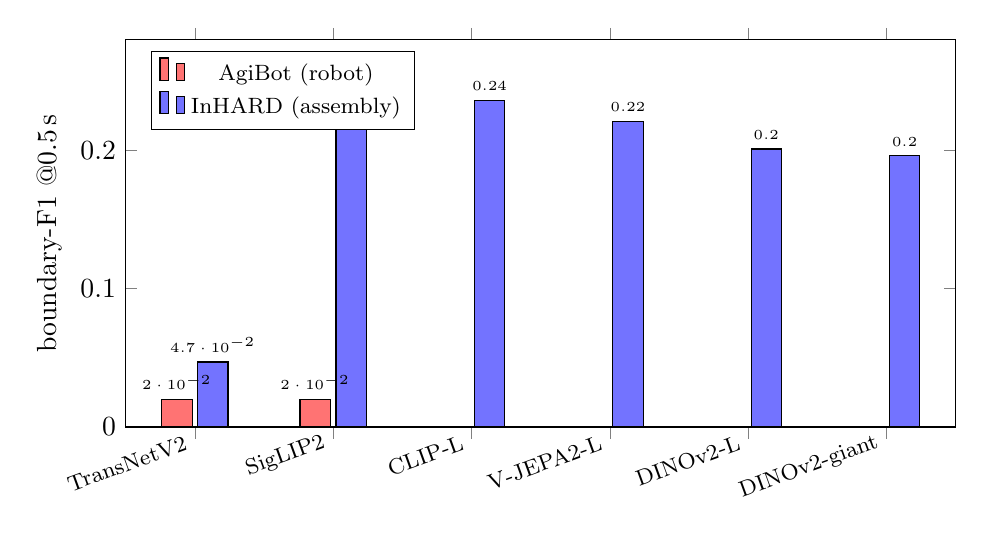
\begin{tikzpicture}
\begin{axis}[
  ybar,
  width=\linewidth, height=6.5cm,
  bar width=11pt,
  ymin=0, ymax=0.28,
  ylabel={boundary-F1 @0.5\,s},
  xtick={1,2,3,4,5,6},
  xticklabels={TransNetV2, SigLIP2, CLIP-L, V-JEPA2-L, DINOv2-L, DINOv2-giant},
  x tick label style={font=\footnotesize, rotate=20, anchor=east},
  nodes near coords, nodes near coords style={font=\tiny},
  legend pos=north west,
  legend style={font=\footnotesize},
  enlarge x limits=0.1,
]
\addplot[fill=red!55] coordinates {(1,0.020) (2,0.020)};
\addplot[fill=blue!55] coordinates {(1,0.047) (2,0.220) (3,0.236) (4,0.221) (5,0.201) (6,0.196)};
\legend{AgiBot (robot), InHARD (assembly)}
\end{axis}
\end{tikzpicture}
\caption{Shot-boundary detection is a domain property, not a harness bug. The same detectors
recover $10$--$12\times$ more boundaries on InHARD's visually varying human-assembly footage than
on AgiBot's fixed-arm/fixed-background robot footage. CLIP-L, V-JEPA2-L, DINOv2-L and DINOv2-giant
were run on InHARD only; DINOv2-giant ($1.1$\,B) is marginally worse than DINOv2-L ($0.3$\,B),
showing that encoder family matters more than parameter count. (Values from the shot-boundary
tables.)}
\end{figure}

\section{Caption grounding: lexical vs.\ semantic}\label{sec:grounding}

Does the caption mention the action the video actually shows? Lexical scoring uses exact
content-word overlap with the GT action text (strict, penalises synonyms). Semantic scoring
splits the caption into clauses and matches each GT action to its best clause by embedding
cosine; recall asks ``is each GT action covered?'' and precision asks ``is each clause the model
wrote actually supported?'' (penalising padding).

\begin{table}[H]
\centering
\caption{AgiBotWorld --- caption grounding (Qwen-2.5-VL-7B).}
\begin{tabular}{lr l}
\toprule
metric & value & what it measures \\
\midrule
Lexical action hit-rate     & 0.086 & fraction of actions with recall $\geq 0.5$ \\
\textbf{Lexical action-F1}  & \textbf{0.107} & headline lexical \\
Semantic recall (MiniLM)    & 0.411 & clause-level meaning match (small encoder) \\
\textbf{Semantic F1 (MiniLM)} & \textbf{0.400} & length-robust headline (small) \\
Semantic recall (BGE)       & 0.616 & clause-level meaning match (large encoder) \\
\textbf{Semantic F1 (BGE)}  & \textbf{0.610} & length-robust headline (large) \\
Granularity-aware recall    & 0.198 & bidirectional containment match \\
\bottomrule
\end{tabular}
\end{table}

\textbf{The lexical--semantic gap is the story.} Lexical action-F1 is only 0.107 but BGE
semantic-F1 is 0.610: Qwen describes the right action (``grasps the object'', ``places it in the
bin'') but rarely reuses AgiBot's exact verbs and nouns. A purely lexical metric would badly
under-rate the captions. The metric is robust by construction --- the correlation between
semantic-F1 and caption length is $-0.069$ (essentially zero), so the score cannot be inflated by
writing more words --- and the two encoders are reported side by side (BGE $0.610 >$ MiniLM
$0.400$) so the result is not silently tied to one embedding model.

\textbf{Cross-domain control on YouCook2.} The same caption harness was run on cooking video,
where every metric is expected to improve if the harness tracks real difficulty.

\begin{table}[H]
\centering
\caption{Cross-domain control: caption harness on robot vs.\ cooking video.}
\begin{tabular}{lrr c}
\toprule
metric & AgiBot (robot) & YouCook2 (cooking) & direction \\
\midrule
\textbf{quality\_score}     & 0.583 & \textbf{0.676} & higher (easier domain) \\
Semantic F1 (BGE)           & 0.610 & 0.665 & better grounding \\
Semantic F1 (MiniLM)        & 0.400 & 0.407 & $\approx$ \\
Lexical action-F1           & 0.107 & 0.246 & $2.3\times$ \\
Unique caption ratio        & 0.713 & 0.945 & less repetition \\
Gemma4 / VCI-7B flag rate   & 0.563 / 0.772 & 0.469 / 0.360 & fewer flagged wrong \\
Judge Cohen's $\kappa$      & 0.108 & 0.148 & judges agree more \\
\bottomrule
\end{tabular}
\end{table}

\textbf{Result confirmed.} Every metric moves in the expected direction: on cooking the captions
are more diverse, better grounded both lexically and semantically, flagged less often, and the
composite \texttt{quality\_score} rises $0.583 \to 0.676$. The harness is neither saturated nor
flat --- it tracks domain difficulty. One honest caveat: the lexical gap stays large in
\emph{both} domains (YouCook2 lexical-F1 0.246 vs.\ semantic-F1 0.665), confirming that lexical
overlap under-rates captions everywhere and the semantic metric is the right headline.

\begin{figure}[H]
\centering
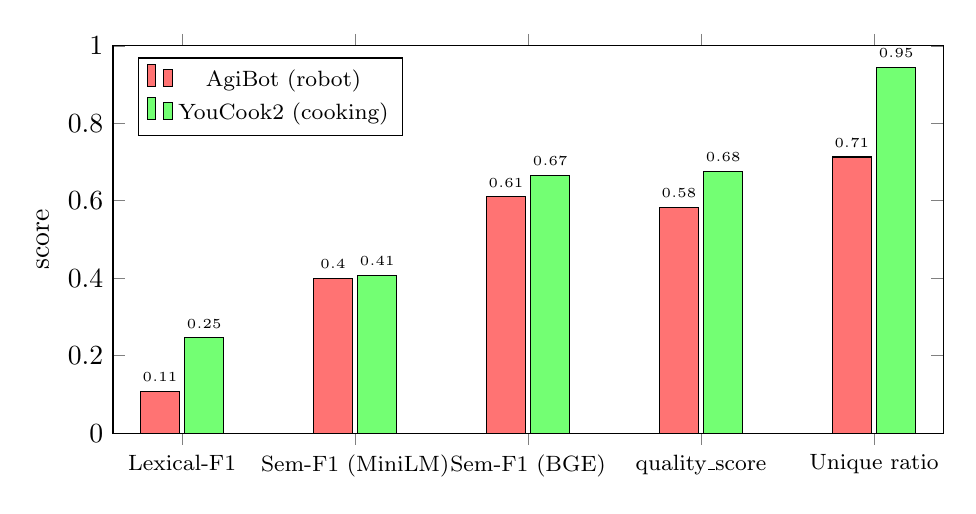
\begin{tikzpicture}
\begin{axis}[
  ybar,
  width=\linewidth, height=6.5cm,
  bar width=14pt,
  ymin=0, ymax=1.0,
  ylabel={score},
  xtick={1,2,3,4,5},
  xticklabels={Lexical-F1, Sem-F1 (MiniLM), Sem-F1 (BGE), quality\_score, Unique ratio},
  x tick label style={font=\footnotesize},
  nodes near coords, nodes near coords style={font=\tiny},
  legend pos=north west,
  legend style={font=\footnotesize},
  enlarge x limits=0.1,
]
\addplot[fill=red!55] coordinates {(1,0.107) (2,0.400) (3,0.610) (4,0.583) (5,0.713)};
\addplot[fill=green!55] coordinates {(1,0.246) (2,0.407) (3,0.665) (4,0.676) (5,0.945)};
\legend{AgiBot (robot), YouCook2 (cooking)}
\end{axis}
\end{tikzpicture}
\caption{Caption metrics track domain difficulty. Every grounding and quality metric is higher on
the easier cooking domain (YouCook2) than on robot video (AgiBot), confirming the harness is
neither saturated nor broken. (Values from the caption-grounding tables.)}
\end{figure}

\section{Judges, consistency, and idle handling}

Two VLM judges watch each window's video and independently flag captions they think are wrong
(no GT is shown to them). A separate consistency block needs no GT at all: it checks whether
neighbouring windows of the same clip agree.

\begin{table}[H]
\centering
\caption{Judge agreement and reference-free consistency (AgiBotWorld).}
\begin{tabular}{lr l}
\toprule
metric & value & meaning \\
\midrule
Gemma4-E4B flag rate    & 0.563 & fraction of captions called wrong \\
VCI-7B flag rate        & 0.772 & fraction of captions called wrong \\
Raw agreement           & 0.585 & fraction both judges agree on \\
\textbf{Cohen's $\kappa$} & \textbf{0.108} & agreement beyond chance \\
Both-incorrect rate     & 0.460 & high-confidence error captions \\
\midrule
Object continuity       & 0.273 & adjacent windows share the object \\
Action continuity       & 0.200 & adjacent windows share the verb \\
Contradiction rate      & 0.053 & clip captions disagree (lower better) \\
Idle-caption recall     & 0.785 & says ``nothing happening'' when idle \\
False-idle on active    & 0.040 & wrongly idle on active (lower better) \\
\bottomrule
\end{tabular}
\end{table}

\textbf{The judges disagree a lot}, and surfacing this honestly is itself a result. VCI-7B flags
77\% of captions, Gemma4 only 56\%, and $\kappa = 0.108$ means agreement is barely above chance;
they catch different failure modes (VCI aggressive, Gemma4 conservative). Using both yields a
high-confidence ``both-incorrect'' set (46\% of windows) far more trustworthy than either alone.
Idle handling works well: genuinely idle windows are labelled idle 78\% of the time and active
windows are wrongly called idle only 4\%, so idle windows do not pollute the action metrics.

\begin{figure}[H]
\centering
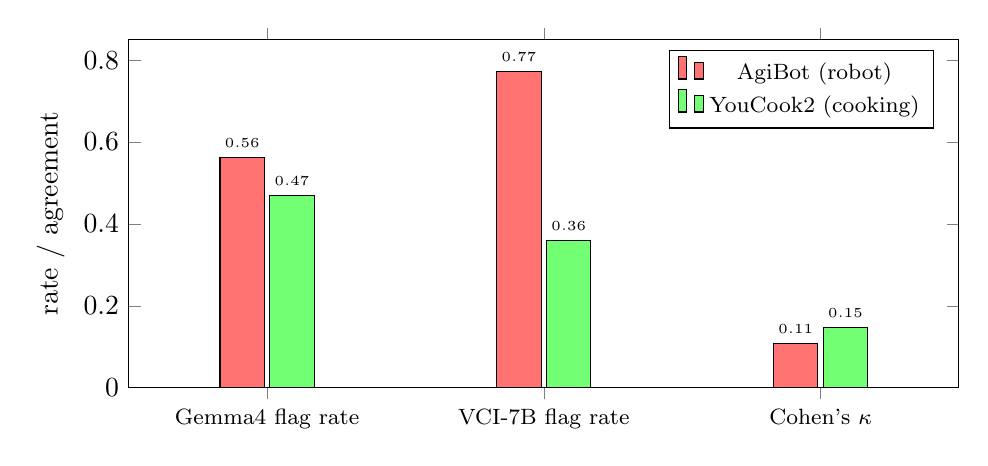
\begin{tikzpicture}
\begin{axis}[
  ybar,
  width=\linewidth, height=6cm,
  bar width=16pt,
  ymin=0, ymax=0.85,
  ylabel={rate / agreement},
  xtick={1,2,3},
  xticklabels={Gemma4 flag rate, VCI-7B flag rate, Cohen's $\kappa$},
  x tick label style={font=\footnotesize},
  nodes near coords, nodes near coords style={font=\tiny},
  legend pos=north east,
  legend style={font=\footnotesize},
  enlarge x limits=0.25,
]
\addplot[fill=red!55] coordinates {(1,0.563) (2,0.772) (3,0.108)};
\addplot[fill=green!55] coordinates {(1,0.469) (2,0.360) (3,0.148)};
\legend{AgiBot (robot), YouCook2 (cooking)}
\end{axis}
\end{tikzpicture}
\caption{Judge flag rates and inter-judge agreement. Both judges flag fewer captions on the
easier cooking domain and agree slightly more ($\kappa$ rises $0.108 \to 0.148$); the low absolute
$\kappa$ on both domains shows the two judges catch different failure modes. (Values from the
judge tables.)}
\end{figure}

\section{Judge comparison against ground truth}\label{sec:judgegt}

The agreement metrics above measure whether the two pipeline judges agree with \emph{each other},
not whether either is \emph{correct}. To measure correctness we use a hand-annotated set of 125
caption windows (AgiBot tasks 327/352/354, balanced: 63 incorrect / 62 correct), where every
Qwen-2.5-VL caption was expert-labelled. Three judges were run on the same windows and scored
against this ground truth; each outputs 1--5 and a caption is flagged when the score is below 5
(positive class = caption error). This is the head-to-head comparison of VCInspector-7B,
Gemma4-E4B, and Qwen-2.5-VL used directly as its own judge.

\begin{table}[H]
\centering
\caption{Judge accuracy vs.\ ground truth (125 hand-annotated windows; Gemma4 on 116, the rest
skipped for too few frames).}
\begin{tabular}{lrrrrrr}
\toprule
judge & N & flag-rate & precision & recall & F1 & accuracy \\
\midrule
\textbf{VCInspector-7B} & 125 & 40.0\% & 82.0\% & 65.1\% & \textbf{0.726} & \textbf{75.2\%} \\
Gemma4-E4B             & 116 & 50.0\% & 65.5\% & 65.5\% & 0.655 & 65.5\% \\
Qwen-2.5-VL (direct)   & 125 & 18.4\% & \textbf{87.0\%} & 31.7\% & 0.465 & 63.2\% \\
\bottomrule
\end{tabular}
\end{table}

\begin{figure}[H]
\centering
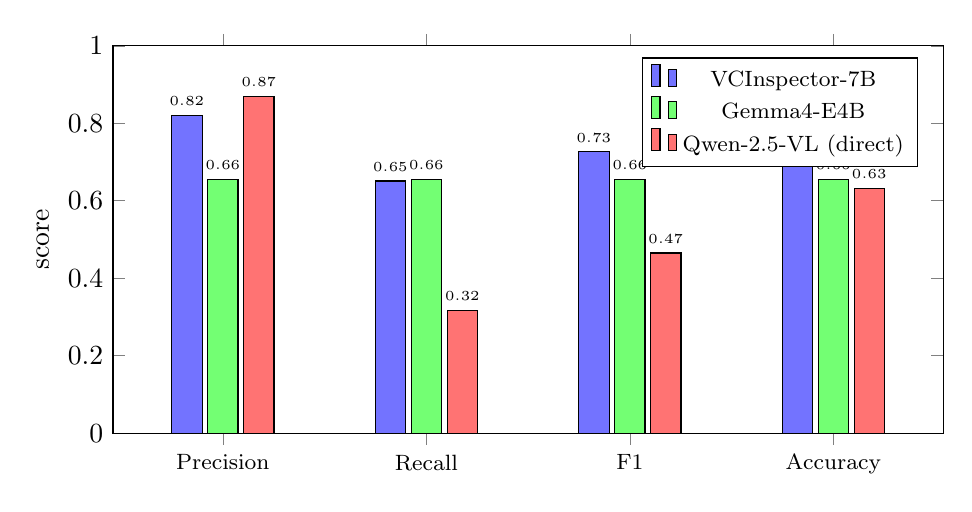
\begin{tikzpicture}
\begin{axis}[
  ybar,
  width=\linewidth, height=6.5cm,
  bar width=11pt,
  ymin=0, ymax=1.0,
  ylabel={score},
  xtick={1,2,3,4},
  xticklabels={Precision, Recall, F1, Accuracy},
  x tick label style={font=\footnotesize},
  nodes near coords, nodes near coords style={font=\tiny},
  legend pos=north east,
  legend style={font=\footnotesize},
  enlarge x limits=0.18,
]
\addplot[fill=blue!55]  coordinates {(1,0.820) (2,0.651) (3,0.726) (4,0.752)};
\addplot[fill=green!55] coordinates {(1,0.655) (2,0.655) (3,0.655) (4,0.655)};
\addplot[fill=red!55]   coordinates {(1,0.870) (2,0.317) (3,0.465) (4,0.632)};
\legend{VCInspector-7B, Gemma4-E4B, Qwen-2.5-VL (direct)}
\end{axis}
\end{tikzpicture}
\caption{Judge correctness against ground truth. VCInspector-7B is best overall (F1 0.726) with
the only balanced precision/recall. Qwen-2.5-VL as its own judge has the highest precision (87\%)
but the worst recall (32\%) --- it flags conservatively and misses most errors. Gemma4-E4B is the
balanced middle. (Values from the offline judge runs.)}
\end{figure}

\textbf{Why only two judges appear in the pipeline benchmark above.} Qwen-2.5-VL-as-judge was an
offline script and was never registered as a pipeline judge plugin, so the full 2{,}587-video run
used the two registered judges (VCInspector-7B and Gemma4-E4B). This section is where the full
three-way, ground-truth-validated comparison lives.

\section{Text--video alignment (reference-free)}

Unlike grounding (caption vs.\ GT \emph{text}), this scores each caption directly against the
\emph{video frames} with SigLIP2 --- no GT needed --- and is the only grounding signal usable when
no GT action text exists. All 15{,}526 windows were scored.

\begin{table}[H]
\centering
\caption{Text--video alignment, AgiBotWorld (SigLIP2).}
\begin{tabular}{lr l}
\toprule
metric & value & meaning \\
\midrule
caption$\leftrightarrow$video sim (mean) & 0.216 & match to frames (std 0.033) \\
GT-text$\leftrightarrow$video sim (mean) & 0.137 & ceiling: how well the correct label grounds \\
caption $-$ GT            & $+0.080$ & caption aligns better than the GT label \\
retrieval median rank    & 387 / 15{,}526 & discriminativeness (random $\approx$ 7{,}763) \\
R@1 / R@10               & 0.004 / 0.034 & rarely finds its own clip exactly \\
within-clip norm.\ rank  & 0.446 & $\approx$ random (0.5) inside a clip \\
\bottomrule
\end{tabular}
\end{table}

Two observations both \emph{confirm} a known limitation rather than contradicting it. First, the
caption scores \emph{higher} against the frames than the GT label does ($+0.080$): SigLIP2 is
web-trained, so a vivid descriptive caption matches the general scene better than a terse GT label
(``grasp''), even when the specific object may be wrong. Second, retrieval is far above random
\emph{globally} (median rank 387 vs.\ 7{,}763) but essentially random \emph{within a clip}
($0.446 \approx 0.5$) --- the encoder can tell a fridge clip from a supermarket clip but cannot
tell two adjacent windows of the same clip apart. This is the familiar ``works at task level,
fails at fine-grained object level'' pattern; text--video is therefore kept as a coarse secondary
check, with the VLM judges and text--text semantic metrics remaining primary.

\begin{figure}[H]
\centering
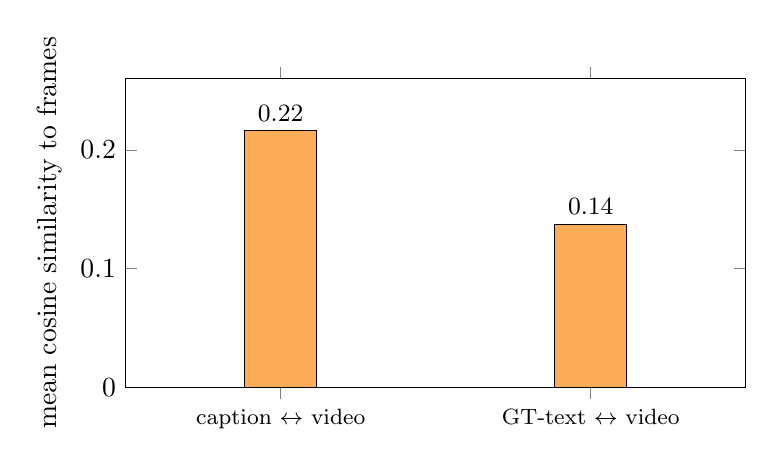
\begin{tikzpicture}
\begin{axis}[
  ybar,
  width=0.78\linewidth, height=5.5cm,
  bar width=26pt,
  ymin=0, ymax=0.26,
  ylabel={mean cosine similarity to frames},
  xtick={1,2},
  xticklabels={caption $\leftrightarrow$ video, GT-text $\leftrightarrow$ video},
  x tick label style={font=\footnotesize},
  nodes near coords, nodes near coords style={font=\small},
  enlarge x limits=0.5,
]
\addplot[fill=orange!65] coordinates {(1,0.216) (2,0.137)};
\end{axis}
\end{tikzpicture}
\caption{Text--video alignment (SigLIP2, AgiBotWorld). The descriptive caption aligns more
strongly with the video frames than the terse GT action label does ($+0.080$) --- an artefact of a
web-trained encoder, which is why this signal is treated as a coarse secondary check. (Values from
the text--video table.)}
\end{figure}

\section{Caption-model comparison: Qwen3-VL-30B (FP8)}\label{sec:qwen3}

A stronger model, Qwen3-VL-30B-A3B-Instruct (FP8), was run on the same 30 test videos and scored
with the same harness and BGE-large semantic encoder. Qwen3-VL initially failed on the A100 GPU
(Ampere has no native FP8; the engine dequantised weights to BF16 at $\sim$60\,GB, exhausting the
40\,GB GPU and leaving 0\,GB for the KV cache). The fix was to run on an \textbf{H100} (native
FP8: weights load at $\sim$31\,GB, leaving ample cache), completing in $\sim$7 minutes. The
two models differ slightly in window count (Qwen3-VL: 120 windows; Qwen-2.5-VL: 125 windows) due
to different fixed-stride runs; results are model-level comparisons, not per-window-identical.

\begin{table}[H]
\centering
\caption{Caption-model comparison: same 30 AgiBot videos, BGE-large semantic scorer.}
\begin{tabular}{lrr c}
\toprule
metric & Qwen-2.5-VL-7B & Qwen3-VL-30B & direction \\
\midrule
\textbf{quality\_score}       & 0.676 & \textbf{0.763} & $+13\%$ \\
Semantic F1 (BGE)             & 0.646 & \textbf{0.659} & better \\
Lexical action-F1             & \textbf{0.205} & 0.202 & $\approx$ \\
Granularity-aware recall      & 0.212 & \textbf{0.246} & better \\
Idle-caption recall           & 0.250 & \textbf{0.429} & $+72\%$ \\
Unique caption ratio          & 0.776 & \textbf{0.867} & more diverse \\
Mean words / caption          & 17.1 & 21.6 & longer \\
sem-F1 length-bias ($r$)      & $-0.547$ & \textbf{$-0.181$} & more robust \\
\bottomrule
\end{tabular}
\end{table}

\textbf{Qwen3-VL-30B wins on every quality dimension.} The composite \texttt{quality\_score}
rises $0.676 \to 0.763$ (+13\%). The biggest gains are not in raw semantic grounding (which
improves modestly, $0.646 \to 0.659$) but in idle-caption recall ($0.250 \to 0.429$ --- the larger
model explicitly says ``nothing is happening'' when appropriate) and caption uniqueness
($0.776 \to 0.867$ --- less verbatim repetition). Lexical F1 is nearly identical ($0.205$ vs
$0.202$), confirming that both models describe the same actions using different vocabulary; the
gain is in diversity and semantic precision, not exact word choice.

A notable structural difference is length-robustness. Qwen-2.5-VL's semantic-F1 correlates
appreciably with caption length ($r = -0.547$): shorter captions score lower, indicating some
gamesmanship by verbosity. Qwen3-VL's correlation is much weaker ($r = -0.181$), suggesting its
longer captions add information rather than padding. The harness's length-robustness diagnostic
surfaces this difference, which a single aggregate score would have hidden.

\begin{figure}[H]
\centering
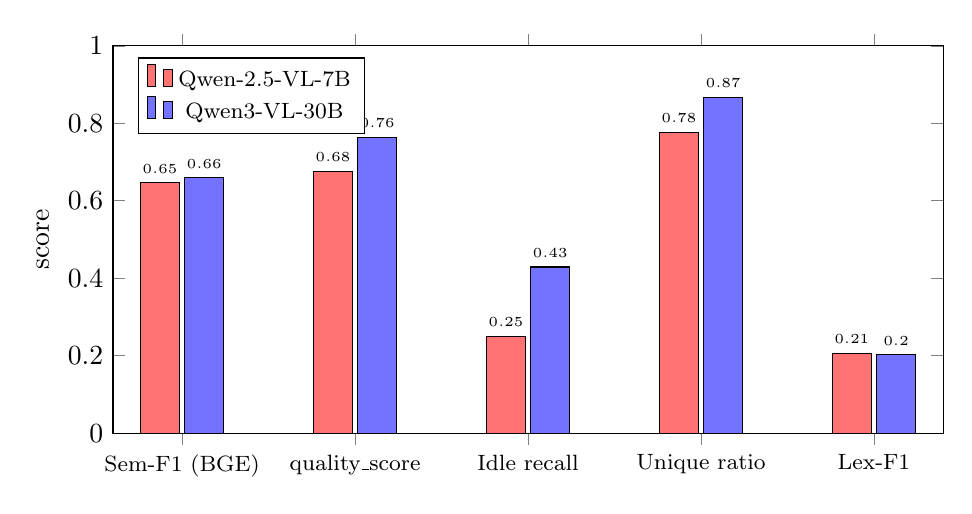
\begin{tikzpicture}
\begin{axis}[
  ybar,
  width=\linewidth, height=6.5cm,
  bar width=14pt,
  ymin=0, ymax=1.0,
  ylabel={score},
  xtick={1,2,3,4,5},
  xticklabels={Sem-F1 (BGE), quality\_score, Idle recall, Unique ratio, Lex-F1},
  x tick label style={font=\footnotesize},
  nodes near coords, nodes near coords style={font=\tiny},
  legend pos=north west,
  legend style={font=\footnotesize},
  enlarge x limits=0.1,
]
\addplot[fill=red!55]  coordinates {(1,0.646) (2,0.676) (3,0.250) (4,0.776) (5,0.205)};
\addplot[fill=blue!55] coordinates {(1,0.659) (2,0.763) (3,0.429) (4,0.867) (5,0.202)};
\legend{Qwen-2.5-VL-7B, Qwen3-VL-30B}
\end{axis}
\end{tikzpicture}
\caption{Caption-model comparison on 30 AgiBot test videos. Qwen3-VL-30B leads on composite
quality ($+13\%$) and idle-caption recall ($+72\%$), with comparable lexical grounding. (Values
from the caption-model comparison table.)}
\end{figure}

\section{Efficiency and caption statistics}

\begin{table}[H]
\centering
\caption{Caption statistics and throughput (AgiBotWorld, Qwen-2.5-VL-7B).}
\begin{tabular}{lr l}
\toprule
statistic & value & note \\
\midrule
Caption windows         & 15{,}526 & one caption per window \\
Unique caption ratio    & 0.713 & lower = more repetitive \\
Mean / median words     & 17.6 / 18 & caption length \\
Vocabulary size         & 923 & distinct words used \\
Most-duplicated caption & $\times$77 & repeated verbatim \\
Caption compute / caption & 0.309\,s & true per-stage compute \\
Est.\ caption tokens / s & 74.2 & throughput proxy \\
\bottomrule
\end{tabular}
\end{table}

\section{Verdict}

The harness behaves exactly as designed and its numbers are internally consistent. Lexical
scores are far below semantic scores (synonym tolerance working); the semantic score is
length-robust (not gameable); idle windows are cleanly separated; the judges' low agreement is
surfaced honestly; and shot detection is shown to be no better than fixed-stride on a
semantic-boundary domain. Crucially, both cross-domain controls succeed: detectors recover
$10$--$12\times$ more boundaries on InHARD's visually varying footage, and the caption metrics
improve across the board on YouCook2's easier cooking domain --- proving the harness measures
genuine difficulty rather than artefacts. For the captions themselves, Qwen-2.5-VL is
semantically decent (BGE semantic-F1 0.61) and self-consistent (5\% contradiction) but lexically
loose and somewhat repetitive (unique ratio 0.71): it gets the action right and the exact object
wording less so. The head-to-head comparison on 30 test videos shows Qwen3-VL-30B
(Section~\ref{sec:qwen3}) is strictly better on the composite \texttt{quality\_score} ($0.676 \to
0.763$, $+13\%$), with the largest gains in idle handling and caption diversity; the trade-off is
that it requires an H100 GPU and produces longer captions. The harness is ready to extend this
ranking to any further model or caption set.

\end{document}
